\section{Resultados}


Após a realização do cruzamento das três bases de dados utilizadas nesse trabalho, resultou-se em um dataframe final com 367.176 linhas.

Dentro do Python, o primeiro procedimento de pré-processamento realizado foi a tratativa dos dados ausentes. Após análise preliminar foi identificado que apenas a variável GRUPO FUNÇÃO possuía valores ausentes ou então valores classificados como N€O INFORMADO, NA0 INFORMADO, NAO INFORMADO ou NAO LOCALIZADO. Essas quatro últimas classificações, na prática, equivalem também a valores ausentes. As linhas nessas situações totalizaram 107.323, que representa 29,23\% da base total. Como essa variável representa a profissão do cliente, optou-se por excluir esses dados da base original, além do que restamos com uma base para aplicação do modelo com tamanho consideravelmente bom, 259.853 linhas.

Ainda nesta etapa foram realizadas análises descritivas sobre as variáveis utilizadas no modelo. Identificou-se, pela análise gráfica (Figura \ref{fig:graf-idade}) e pelo conhecimento do negócio, que idades a partir de 25 anos e inferiores a 80 anos estão mais propícias à finalização da venda.

\begin{figure}[h]
\captionsetup{labelfont=bf,size=normalsize}
    \centering
     \includegraphics[scale=0.4]{Grafico-Idade.png}
\caption{Distribuição da Variável Idade dos Clientes.} {\footnotesize Fonte: Elaborado pelo Autor, 2022.}
\label{fig:graf-idade}
\end{figure}

Com isso, optou-se por manter na base de dados apenas os clientes com idade maior ou igual a 25 anos e com menos de 80 anos, resultando em um dataframe com 257.939 linhas.

Da base final avaliou-se que apenas 0,72\% dos dados são da categoria de venda (Figura \ref{fig:graf-rotulo}), que é o nosso interesse em classificação. Isso representa uma base desbalanceada, o que necessita de técnicas específicas para o momento de execução do modelo de classificação. Para o próximo semestre essas técnicas serão avaliadas.

\begin{figure}[H]
\captionsetup{labelfont=bf,size=normalsize}
    \centering
     \includegraphics[scale=0.7]{Grafico-Rotulo.png}
\caption{Distribuição da Classificação dos Clientes (Rótulo).} {\footnotesize Fonte: Elaborado pelo Autor, 2022.}
\label{fig:graf-rotulo}
\end{figure}

Dentre os clientes analisados, 54,86\% são do sexo Feminino e 45,14\% do sexo Masculino (Figura \ref{fig:graf-sexo}).

\begin{figure}[H]
\captionsetup{labelfont=bf,size=normalsize}
    \centering
     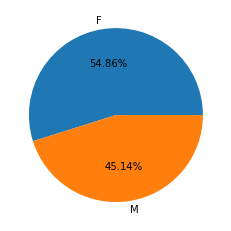
\includegraphics[scale=0.7]{Grafico-Sexo.png}
\caption{Distribuição da Variável Sexo dos Clientes.} {\footnotesize Fonte: Elaborado pelo Autor, 2022.}
\label{fig:graf-sexo}
\end{figure}


É possível notar também que a grande maioria dos clientes, 81,97\%, estão localizados nos estados de Rio de Janeiro e Bahia (Figura \ref{fig:graf-estado}).

\begin{figure}[H]
\captionsetup{labelfont=bf,size=normalsize}
    \centering
     \includegraphics[scale=0.7]{Grafico-Estado.png}
\caption{Distribuição dos clientes segundo seu Estado.} {\footnotesize Fonte: Elaborado pelo Autor, 2022.}
\label{fig:graf-estado}
\end{figure}


Além disso, 28,50\% dos clientes possuem a profissão de Professor, seguido pela profissão de Polícia, 17,08\%. Na figura \ref{fig:graf-prof} é possível avaliar o ranking das dez principais profissões dos clientes na base de dados.

\begin{figure}[H]
\captionsetup{labelfont=bf,size=normalsize}
    \centering
     \includegraphics[scale=0.7]{Grafico-Profissao.png}
\caption{Distribuição das 10 principais profissões dos clientes.} {\footnotesize Fonte: Elaborado pelo Autor, 2022.}
\label{fig:graf-prof}
\end{figure}

Para a próxima etapa do trabalho serão realizadas análises descritivas mais detalhadas envolvendo os principais perfis dentro dos clientes que efetivaram suas vendas, além de ajustes que se façam necessários na base atualmente definida como Base Final.